\documentclass[a4paper,12pt]{article}
\usepackage[osf]{mathpazo}
\usepackage{ms}
\usepackage{amsmath,amsfonts,amssymb}
\usepackage{natbib}
\usepackage{lineno}
\usepackage{graphicx}
\usepackage{caption}
\modulolinenumbers[5]
\linenumbers

\pdfminorversion=3

\makeatletter
\renewcommand{\@biblabel}[1]{\quad#1.}
\makeatother

\title{Statistical and conceptual challenges in the comparative analysis of principal components}
\author{
Josef C. Uyeda$^{1,*}$, Daniel S. Caetano$^1$, and Matthew W. Pennell$^1$
}

\date{}
\affiliation{
 $^{1}$ Department of Biological Sciences \& Institute for Bioinformatics and Evolutionary Studies, University of Idaho, Moscow, ID 83844, U.S.A.\\ 
 $^{*}$ Email for correspondence: \texttt{pseudacris@gmail.com}\\
}

\runninghead{PCA in comparative analyses}
\keywords{Phylogenetic comparative methods, principal components, Brownian motion, Ornstein-Uhlenbeck, multivariate statistics}


\begin{document}

\mstitlepage
\parindent=1.5em
\addtolength{\parskip}{.3em}
\vfill

\section{Abstract}
\begin{enumerate}
\item A common procedure when analyzing multivariate data in a phylogenetic framework is to first transform the data into a set of principal component (PC) axes. Techniques for ``correcting for phylogeny'' when computing PCs have been developed and applied widely in the empirical literature. However, standard (i.e., uncorrected) principal components continue to be widely used in comparative analyses.

\item We demonstrate that failing to include phylogenetic relationships when calculating PC scores will mislead inferences in a predictable manner. Specifically, even when data are simulated under Brownian motion (BM), the first several PC scores will appear to have evolved rapidly early in a clade's history and slowed down towards the present day.

\item The primary method for calculating ``phylogenetically corrected'' PC scores relies on the assumption that the traits have evolved under a multivariate BM model. It is unknown whether this assumption is reasonable if the actual traits have evolved under more complex scenarios. Using simulations, we find that for many common models of evolution, calculating PC scores based on a BM model is a reasonable approximation though the first few axes will show inflated support for the true model and the reduced support for the true model in higher components.

\item \emph{Synthesis:} While incorporating phylogeny when calculating PC scores does remove bias in many cases, a more fundamental issue remains when analyzing PCs in a comparative framework --- that drawing meaningful evolutionary inferences from models fit to PCs is challenging. Alternatives approaches for modeling multivariate data on a phylogeny are likely to be more informative, though further statistical and conceptual innovations will be necessary for these to be more broadly applicable.
\end{enumerate} 

\newpage

\section{Introduction}
The units of measurements are not neutral or arbitrary; different ways of representing the same set of data can change the meaning of the measurements and alter the interpretations of subsequent statistical analyses \citep{Hand2004, HansenHoule2008, Houle2011}. Therefore, careful attention needs to be paid to how data is measured and how it is transformed. Furthermore, this should be done with the scientific question in mind in order to ensure that resulting inferences are meaningful \citep{Houle2011}. 

Most approaches for studying evolution in a phylogenetic comparative framework were developed for univariate data \citep[reviewed in][]{PennellHarmon}. Even classical approaches for testing for correlated evolution across a phylogeny \citep[e.g.,][]{Felsenstein1985, Grafen1989, HarveyPagel1991} fundamentally model each trait as having evolved under a process that is independent of the state of the other \citep{HansenOrzack2005}. However, the traits that we are actually interested in studying have likely evolved in concert with a suite of other traits and considering each trait in isolation may give a distorted picture of reality. Therefore, it is often desirable to reduce the multivariate dataset into a set of linear combinations of traits that are orthogonal to one another, such that each linear combination can then be independently analyzed with common comparative methods.

The most common method for reducing the dimensionality of the dataset is to perform Principal Components Analyses (PCA) prior to analyzing the data using phylogenetic comparative methods. The first PC axis is the eigenvector in the direction of greatest variance, the second PC axis, the second greatest variance, and so on. However, standard methods for calculating PC scores assume that the samples are independent of one another, which is hardly ever the case for comparative data. This fact is of course, now almost universally recognized by biologists and conducting comparative analyses without considering the phylogenetic relationships of species is anathema to most evolutionary biologists.
%% Excluded: "As a result of shared common ancestry, relatives are likely to share many traits and trait combinations."

However, the necessity of considering phylogeny in some types of data transformations \citep{Revell2008} is not similarly recognized. Many recent publications still show comparative analyses using standard PCs and thus inadvertently introduce substantial bias into the analyses. Typical examples of traits where this is done include geometric morphometric landmarks \citep[e.g.,][]{Dornburg2011, Hunt2013}, measurements of multiple morphological traits \citep[e.g.,][]{Harmon2010, BergmannIrshick2012, Weir2012, Pienaar2013, Price2014}, and climatic variables \citep[e.g.,][]{KozakWiens2010, Schnitzler2012}. We stress that the papers that we have cited here are simply examples picked haphazardly from a substantial number of papers where this non--intuitive mistake was made.
%% Modified: "Many researchers --- most of whom would never consider analyzing comparative data in a non--phylogenetic context --- continue the practice of conducting comparative analyses on standard PCs and thus inadvertently introduce substantial bias into their analyses." -> This statement is part irrelevant and have a format that sounds aggressive. Do you know what researchers think? Better to focus critics in the research and not the researchers.
%% Modified: haphazardly seems better than "more-or-less random". In sampling means without pattern, but not assure randomness. 

Fortunately, multiple potential solutions exist to address the problem that trait combinations are not phylogenetically independent.  One frequently used method is that of \citet{Revell2008}, who developed a procedure (explained in detail below) for converting multivariate data into ``phylogenetically corrected'' PC axes (hereafter, pPCA), by assuming that the original data evolved along the phylogeny under a multivariate Brownian motion \citep[BM;][]{Edwards1964, Felsenstein1973} model of evolution. In a brief simulation study, \citet{Revell2008} demonstrated that if the underlying model for the traits was indeed a multivariate BM model, performing standard PCA gave biased estimates of the eigenvalues, whereas pPCA removed this bias.

In this brief contribution, we first extend the argument of \citet{Revell2008} and demonstrate that not only are the eigenvalues obtained from PCA biased but that they are biased in a systematic and predictable way. Performing comparative analyses on standard PC axes positively misleads inference. This point has been made in other fields that deal with autocorrelation between observations, such as population genetics \citep{Novembre}, ecology \citep{Podani2002}, climatology \citep{Richman1986} and paleobiology \citep{Bookstein2012}. However, the connection between these previous results and phylogenetic comparative data has not been explicitly made and standard PCs continue to be widely used in the field. We hope that our paper helps change this practice.

Second, as stated above, \citet{Revell2008} assumed that the measured traits had evolved under a multivariate BM model. This has the potential to introduce an odd circularity into the analysis. If we assume that the underlying traits have evolved under BM and calculate a set of pPC axes, it seems reasonable to suppose that if the true model of trait evolution were different, systematic biases in deviations from the BM model could generate predictable distortions across pPC scores. Such distortions could affect inference of models of trait evolution and parameters values. To our knowledge, the effect of this bias has not been explored. We perform a simulation study to investigate this question.
%% Modified: "If we assume that the underlying traits have evolved under BM and calculate a set of pPC axes based on this assumption, it seems reasonable to suppose that if the true model of trait evolution were different, systematic biases in deviations from the BM model could generate predictable distortions across pPC scores that could affect inference of models of trait evolution."

Last, we consider the interpretation of evolutionary models fit to pPC axes and discuss the conceptual and statistical advantages and disadvantages of using pPCA compared to alternative approaches for studying multivariate evolution in a phylogenetic comparative framework.

\section{Methods}
\subsection{\emph{Overview of pPCA}}
Before describing our analyses, we briefly overview the approach of \citet{Revell2008} for computing pPC scores for each species. In conventional PCA, a $m \times m$ covariance matrix $\mathbf{R}$ is computed from a matrix of trait values $\mathbf{X}$ for the $n$ species and $m$ traits
\begin{equation}\label{eq:rpca}
\mathbf{R} = (n-1)^{-1}(\mathbf{X} - \mathbf{1m}^\intercal)^\intercal (\mathbf{X} - \mathbf{1m}^\intercal)
\end{equation}
where $\mathbf{m}$ is a vector containing the means of all $m$ traits and $\mathbf{1}$ is a column vector of 1s. We note that in many applications $\mathbf{X}$ may not represent the raw trait values; in geometric morphometrics, for example, size, translation and rotation will often be removed from $\mathbf{X}$ prior to computing $\mathbf{R}$ \citep{RohlfSlice, Bookstein1997}. The eigenvalues $\mathbf{D}$ and eigenvectors $\mathbf{V}$ of $\mathbf{R}$ are then obtained using singular--value decomposition $\mathbf{R}=\mathbf{V}\mathbf{D}\mathbf{V}^{-1}$ or some related technique. The scores $\mathbf{S}$, the trait values of the species along the PC axes are computed as
\begin{equation}\label{eq:Spca}
\mathbf{S}=(\mathbf{X} - \mathbf{1m}^\intercal)\mathbf{V}.
\end{equation}

Phylogenetic PCA differs from this procedure in two important ways \citep{Revell2008,Polly2013} . First the covariance matrix is inversely weighted by the expected covariance of trait values between taxa under a given model $\mathbf{\Sigma}$. Under a BM model of trait evolution, $\mathbf{\Sigma}$ is simply proportional to the matrix representation of the phylogenetic tree $\mathbf{C}$, such that $\Sigma_{i,j}$ is the shared path length between lineages $i$ and $j$. Including the expected covariance between trait values essentially just re--orients the axes according to the phylogeny. Second, the space is centered on the ``phylogenetic means'' $\mathbf{a}$ of the traits rather than the arithmetic means. In pPCA, Equation \ref{eq:rpca} is therefore modified as
\begin{equation}\label{eq:rppca}
\mathbf{R} = (n-1)^{-1}(\mathbf{X} - \mathbf{1a}^\intercal)^\intercal \mathbf{\Sigma}^{-1} (\mathbf{X} - \mathbf{1a}^\intercal)
\end{equation}
where $\mathbf{a}=[(\mathbf{1}^\intercal \mathbf{\Sigma}^{-1} \mathbf{1})^{-1} 
\mathbf{1}^\intercal \mathbf{\Sigma}^{-1} \mathbf{X}]^\intercal$ \citep{RevellHarmon2008,Revell2008}. Similarly, $\mathbf{S}$ can be calculated for pPCA using Equation \ref{eq:Spca} but substituting the phylogenetic means for the arithmetic means
\begin{equation}\label{eq:Sppca}
\mathbf{S}=(\mathbf{X} - \mathbf{1a}^\intercal)\mathbf{V}
\end{equation}
where again, $\mathbf{V}$ is a matrix containing the eigenvectors of $\mathbf{R}$ (in this case obtained from Equation \ref{eq:rppca}).

Three things are worth noting about the properties of pPCA. First, both PC and pPC axes are all orthogonal to one another. Second, unlike PCA, the scores of each pPC axis are not orthogonal to scores on other axes. Third, while the eigenvectors and eigenvalues of pPCA are indeed phylogenetically independent (assuming the model used to construct $\mathbf{\Sigma}$ is appropriate), the scores themselves are not \citep{Revell2008, Polly2013}. Both these properties imply that when testing for correlated evolution among pPC scores or between pPC scores from one axis an another trait, it is necessary to perform a phylogenetic analyses, just as one would with any other trait \citep{Revell2008, Polly2013}.
%% Modified: The first part of the paraghraph was very confusing. Changed to make clearer.


\subsection{\emph{Simulations}}
\subsubsection{Effect of PCA on model selection under multivariate Brownian motion}
We simulated 100 replicate datasets under multivariate Brownian motion to evaluate the effect of using standard versus phylogenetic PCA to infer the mode of evolution. For each dataset, we used \texttt{TreeSim} \citep{treesim} to simulate a phylogeny of 50 terminal taxa under a pure--birth process and scaled each tree to unit height. We then simulated a 20--trait dataset under multi-variate Brownian motion. For each simulation, we generated a positive definite covariance matrix for the multivariate BM process $\mathbf{\Sigma}$, by drawing eigenvalues from an exponential distribution with a rate $\lambda = \text{1/100}$ and randomly oriented orthogonal eigenvectors. We then used this matrix to sample a covariance matrix for the tip states $\mathbf{X}\sim \text{mvNorm}(\mathbf{0}, \mathbf{C} \otimes \mathbf{\Sigma})$.

For each of the 100 simulated datasets, we computed PC scores using both standard methods and pPCA \citep[with the \texttt{phytools} package][]{phytools}. Then we used \texttt{phylolm} \citep{HoandAne2014} to fit models of trait evolution to the original data and to all PC scores obtained by both methods. Following \citet{Harmon2010}, we considered three models of trait evolution: 1) BM; 2) Ornstein--Uhlenbeck with a fixed root \citep[OU;][]{ Hansen1997}; and 3) Early Burst \citep[EB;][]{Blomberg2003, Harmon2010}. We then calculated the Akaike weights (AICw) for each model/transformation/trait combination.

\subsubsection{Effect of using PCA when traits are not Brownian}
We conducted an additional set of simulations in which we varied the underlying model for each of the traits in the dataset. Because of difficulties in efficiently simulating large multivariate datasets of covarying traits under OU or EB models, we instead simulated 20 independent traits under BM, OU and EB for 50 taxa trees (as above, but setting all eigenvalues equal to one another). Of course, this is certainly not represenative of the process that have shaped real multivariate data, considering this simple case allowed us to investigate how misspecifying the model of trait evolution can impact analyses under the simplest scenario.
%% Suggestion: The Carnivora climate dataset is strongly OU. We can notice the effect of PCA vs. pPCA in the parameter estimates. This is an example of a true (very) covariate set of traits.

For the BM simulations, we set $\sigma^2=\text{1}$. For OU, we set $\sigma^2=\text{1}$ and $\alpha=\text{2}$, such that the phylogenetic half--life \citep[log(2)/$\alpha$;][]{Hansen2008} was equal to $\sim$ 0.35 of the total tree depth. For EB, we again set $\sigma^2=\text{1}$ and set $a$, the exponential rate of deceleration, to be log(0.02). 

As above, we fit BM, OU and EB models to the original data, PC scores and pPC scores for each simulated dataset and estimated parameters and AICw. In addition to the model--fitting and comparison, for every transformation, we applied two common diagnostic tests for deviation from BM--like evolution to all trait/PC axes. First, we fit a linear model between the absolute size of the contrats \citep{Felsenstein1985} and the height of the node at which they were calculated \citep[i.e., the ``node height test'' of][]{FreckletonHarvey2006}. Second, we characterized the disparity through time \citep{Harmon2003} using the \texttt{geiger} package \citep{geiger2}. All simulations and analyses were conducting using R v3.0.2 \citep{R}.


\subsection{\emph{Empirical examples}}
We used morphometric data for the Felidae and climate data for the Carnivora to test the effect of standard PCA and pPCA in empirical datasets. In both analyses we used the Carnivora supertree by \cite{Nyakatura_2012} and pruned species that were not present in each dataset. Felidae measurements are the compilation of two independent sources --- five cranium measurements from \cite{slater_2009} and body mass and skull width from \cite{sakamoto_2010} (Online Supplementary table). We obtained geographical distribution for Carnivora species from GBIF database (\textit{Citation}) and world-wide climate data with 2.5 arc--minutes resolution from \cite{hijmans_2005}. Again, we fit BM, OU and EB models to the original data, PC and pPC scores. We also did the same diagnostic tests for deviation from BM described above.

\section{Results}
\subsection{\emph{Simulations}}
\subsubsection{Effect of PCA on model selection under multivariate Brownian motion}
Standard PCA introduces a systematic bias in the favored model across principal components. In our simulations, EB models had systematically elevated support as measured by Akaike weights for the first few components, for which it generally exceeded support for the BM model (Figure \ref{corbm}). Fitting models sequentially across PC axes 1--20 revealed a regular pattern of increasing support for BM models moving from the first toward the intermediate components, followed by increasing support for OU models among later components (which generally approached an AICw of 1). This regular pattern across trait axes was not present for either the original datasets, or for phylogenetic principal components, which found strong support for the BM model regardless of which trait was analyzed. (We note that the theoretical maximum for Akaike weights for the BM model is $\sim 0.576$, as BM is a special case of the OU and EB models when $\alpha=0$ or $a = 0$, respectively, and cannot have a higher likelihood than either of these models).   

\subsubsection{Effect of using PCA when traits are not Brownian}
If the underlying model was either OU or EB rather than BM, then phylogenetic PCA tended to increase support for the true model relative to the original trait variables for the first few component axes (Figures \ref{aicwbm}, \ref{aicweb}, \ref{aicwou}, in Supplementary Online Material). For example, when each of the original trait variables were simulated under an OU process, support for the OU model increased for pPC1 relative to the original trait variables. Higher principal component axes inferred a regular pattern of decreasing support for the OU model, with the last few PCs have equivocal support for either a BM or OU model (Figure \ref{oufit}, top panel). Furthermore, parameter estimation was affected by phylogenetic PCA. $\alpha$ was over--estimated for the first few pPC scores and underestimated for the higher components until the estimated value was essentially equivalent to 0 (Figure \ref{oufit}, bottom panel). 
%% Comment: There is no difference in the support for the true model between PCA and pPCA when the true model is EB. The pattern is the same, strong support for the true model in the first axes and poor in the last ones. This is evident in the figure but is not mentioned in the text. Need to add discussion of the EB pattern.

Examining the results from the node--height tests (Figure \ref{nhplot}) and the disparity through time analyses (Figure \ref{dttplot}) help clarify the results we observed from model comparison and parameter estimation. 
Under OU models, traits are expected to have the highest contrasts near the tips, whereas under EB models, traits will have the highest contrasts near the root of the tree. Standard PCA tends to select linear combinations of traits that maximize the contrasts at the root of the tree, thereby maximizing the overall variance explained across the entire dataset. Thus, the first few PCs are skewed toward resembling EB models, while the last few PCs are skewed toward resembling OU models. By contrast, the effect of pPCA on the node--height relationship depends on the generating model. When traits are evolved under an OU model, the first few pPC axes show an exaggerated pattern of high variance towards the tips. Likewise, when traits are evolved under an EB model, the first few pPC axes show an exaggerated pattern of high variance towards the root of the tree. For traits generated under both OU and EB models, the higher components resemble BM--like patterns. To summarize, the first few pPC axes calculated on traits evolved under an OU process appear to be even more OU--like than the original traits. Similarly, if the true model is EB, the first few pPC axes will resemble an even more extreme EB model.

\subsection{\emph{Empirical examples}}
Both the analysis of morphological and climate data showed patterns that corroborate results from simulations. Morphometric measurements from Felidae species are homogeneously BM--like across all traits. While body mass showed strong correlation (0.81) with the highest axis of variation (PC$1$) under standard PC transformation. The first PC under pPCA is similarly strong correlated ($>$0.9) with all seven traits. When the direction of phylogenetic covariation is added to the PC transformation, the relative contribution of body mass to PC$1$ is substantially diminished. This scenario makes biological interpretation of the PC axis especially difficult, since PC$1$ cannot be related to a single trait (see Discussion). Standard PCA shows clear support for the OU model in the last four axes --- similar to BM simulation. On the other hand, the first three axes have mixed support for BM and OU models. The first and third axes favour BM and the second OU. Phylogenetic PC show mixed support for BM and OU models across all axes. This result contrasts with the homogeneous support for the true model found in the BM simulated data transformed with pPCA. This is somewhat expected, since evolutionary patterns among traits could be better explained by different models and empirical data frequently show more support to OU models \citep{Harmon2010}.

Climate data among Carnivora species showed strong correlation among its variables. Under standard PCA the highest axis of variation is correlated with temperature seasonality (0.98), followed by annual precipitation (-0.84; i.e., inversely correlated) in PC$2$. The pPCA first axis is highly correlated with temperature seasonality (0.99), temperature annual range (0.94) and minimum temperature of coldest month (-0.82). Unlike the OU simulated dataset, climate variables showed exclusive support for the OU model across all traits in the original data and PC axes, both for PCA and pPCA. Although there is no trend in the supported model, we verified that estimated values for $\alpha$ across PC axes differ among data transformations. Standard PCA results in low $\alpha$ values (higher phylogenetic half--life) in the first PC axes and high $\alpha$ values (lower phylogenetic half--life) for the last axes. This pattern is expected, since most of the divergence in the first axes happen towards the root of the phylogeny and the last axes concentrate the changes towards the tips. This trend is not observed when applying pPCA to the data. Values of $\alpha$ estimated to the axes of pPCA show a pattern similar to the same parameter estimates for the original climate data. Both low and high values of $\alpha$ are found among the first and last PC/traits.

\section{Discussion}
\subsection{\emph{Standard PCA should not be used for comparative analyses}} 

The effect of computing PC scores on phylogenetically correlated data has not been widely appreciated, probably because PCA is viewed as a neutral linear transformation of multivariate data. Certainly, when used as a descriptive tool, PCA can be broadly used even when assumptions regarding statistical non--independence or multivariate normality are violated \citep{Jolliffe2002}. Thus, there is nothing inherently wrong with using standard PCA or pPCA on comparative data to describe axes of maximal variation across species or for visualizing divergence across phylo--morphospace \citep{Sidlauskas2008}. However, we demonstrate that using PCA for inference from non--independent observations is considerably more problematic \citep{Jolliffe2002}. This conclusion is not limited to comparative data \citep[see][]{Richman1986, Podani2002, Novembre, Bookstein2012}. For example, \citet{Novembre} demonstrated that apparent waves of human migration in Europe obtained from PCA of genetic data \citep[e.g.,][]{Cavalli} could be attributed to artifacts similar to those we document here (in their case, it was geographic structure, rather than phylogenetic structure). And while the bias introduced by applying standard PC to comparative data has been documented previously \citep{Revell2008, Polly2013}, we have tried to emphasize just how these biases affect inferences that evolutionary biologists care about.

An intuitive way to think about the effect of PCA is to consider a multivariate BM process on a phylogeny. Despite a constant rate of evolution across each dimension of trait space, stochasticity will ensure that some dimensions will diverge more rapidly than expected early in the phylogeny, while others will diverge less. All else being equal, dimensions that happen to diverge early are expected to have the greatest variance across species, and standard PCA will identify these axes as the primary axes of variation. However, once these trait axes are selected, ``regression toward the mean'' ensures that the chance elevation of rates that occurred early on in the phylogeny is unlikely to be maintained, resulting in a characteristic ``Early--Burst'' pattern of evolution for the first few principal components \citep[for a related point, see][]{Pennell2012}.
%% Suggestion: The above phrase is "complicated". It is confusing if "selected" means the process of selection of axes during the evolution of the group or the PC axis selected by PCA? "Regression toward the mean" could also be better explained. Seems better to split into two phrases and add more detail.
An analogous process will result in the last few PCs following an OU process, in which the amount of divergence will appear to increase toward the present. Standard PCA thus ``sorts'' orthogonal trait dimensions by whether they follow EB, BM and finally, OU like patterns of trait divergence. Thus, meaningful inferences regarding either slow--downs or accelerations of trait evolution cannot be made from univariate PC scores inferred from standard PCA. 

These results certainly do not imply that the biological inferences made from analyzing standard PC scores in a comparative framework are necessarily incorrect. %Effect may be small when low dimensional
Interestingly, when \citet{Harmon2010} analyzed the evolution of PC2 (what they referred to as ``shape'') obtained using standard PCA, they found very little support for the ``Early Burst'' model \citep{Blomberg2003} across their 39 datasets. The fact that their use of standard PC axes biased their results \emph{towards an ``Early Burst'' pattern} only serves to strengthen their overall conclusion that such slowdowns are indeed rare \citep[but see][]{SlaterPennell}. However, our results do suggest that in some cases, analyses conducted with PC axes should perhaps be revisited to ensure that results are robust.

\subsection{\emph{Using pPCA when trait evolution is non-Brownian}}
In his original pPCA method, \citet{Revell2008} assumed that the original traits evolved under a multivariate BM model. Under this assumption, phylogenetic PCA mitigates the biased selection of PC axes by scaling divergence by the expected divergence given the branch lengths of the phylogeny. When the true model of evolution is not BM, then systematic deviations will be magnified by pPCA, and result in predictable distortions across pPC axes. We find that these distortions primarily serve to inflate the support for the true model of trait evolution when all dimensions follow a common model, which, in and of itself, is not necessarily suboptimal behavior (just as we expect greater signal in larger datasets). However, regular and predictable distortions across trait axes confound interpretation of the evolutionary model and estimated parameters (Figures \ref{nhplot} and \ref{dttplot}). Of course when we analyze real data, we do not know what the true model is and so the effects of model misspecification are difficult to quantify for a given dataset. At a minimum, it seems likely that regular changes in evolutionary tempo and mode should be expected when progressing from one pPC axis to the next, merely as a result of model misspecification and the biased selection of stochastic events into particular pPC axes.

\cite{Revell2008} suggested that alternative covariance structures could be used to estimate phylogenetically independent PCs for different models. For example, one could first optimize the $\lambda$ model \citep{Pagel1999} across all traits simultaneously and then rescale the branch lengths of the tree according to the estimated parameter in order to obtain $\mathbf{\Sigma}$ for use in Equation \ref{eq:rppca}. However, one cannot compare model fits across alternative linear combinations of traits so the data transformation must be separate from the model--based inference.  Furthermore, as noted by \citet{Revell2008}, parameters estimated to construct the covariance structure for the pPCA will likely be different from the same parameters estimated using the PC scores themselves. Additionally, this procedure is restricted to models that assume a shared mean and variance structure across traits \citep[see][for examples where this does not apply]{Hansen2008, Bartoszek2012}. As such, if one is to use pPCA to transform trait data, it is necessary to make some simplifying and rather ad--hoc assumptions and hope that inferences are generally robust to these decisions.

\subsection{\emph{The interpretation of pPCA}}

Aside from the statistical issues raised here, a broader, and more interesting, question is how one should draw evolutionary inferences from models of trait evolution fit to pPC axes. While principal components are convenient representations of multivariate data in univariate space, this comes at the cost of abstracting the data that is analyzed from the questions that are asked. 

First, using principal components often divorces model fitting from the study of interpretable evolutionary processes. If we treat the PC scores as a univariate trait, we are only considering divergence along the PC axis. This is sensible from a purely statistical standpoint but in doing so, we may miss a great deal about what is actually going on in the data. The first principal component axis computed from comparative data is the major axis of divergence across a clade (also known as the ``line of divergence''). This axis is of considerable interest in evolutionary biology. The direction of this line of divergence may be affected by the orientation of within--population additive genetic (co)variance $\mathbf{G}$, such that evolutionary trajectories may be biased along ``genetic lines of least resistance'' \citep[i.e., divergence occurs primarily along the leading eigenvector of $\mathbf{G}$, $G_{\text{max}}$;][]{Schluter1996}. Alternatively, the line of divergence may align with the ``selective lines of least resistance'', due to the structure of phenotypic adaptive landscapes \citep{Arnold2003, Jonesetal2007, Arnoldetal2008}, or else may be driven by patterns of gene flow between populations \citep{Guillaume2007} or the pleiotropic effects of new mutations \citep{Jonesetal2007, Hether2013, Houle2013}. Furthermore, pleiotropy and the genetic covariance between traits has been proposed as a potential resolution to the ``paradox of stasis'' \citep{HansenHoule2004}; traits with abundant within--population additive genetic variation may be constrained over macroevolutionary time scales \citep{WalshBlows2009}. Phylogenetic comparative data can potentially provide unique and novel insights into the connection between micro-- and macroevolution \citep{Hohenlohe2008} but such questions can only be addressed in a truly multivariate context. While the traits identified by PCA will be statistically orthogonal (assuming that the model of evolution used for the transformation is appropriate; see above), this is only true in the particular snapshot captured by comparative data and should not be taken as sufficient evidence to conclude that they are evolving independently.

For some macroevolutionary questions, evolutionary processes may not be of primary interest and the loss of information when using PCs may be acceptable. For instance, if the goal of fitting and comparing models is to make broad inferences about evolutionary patterns, such as the ``rate'' of trait evolution \citep{Freckleton2011, Hunt2012}, then we may not care if the models are connected to any process. Many commonly used trait models \citep[notably, the ``Pagel'' tree transformations $\lambda, \delta, \kappa$;][]{Pagel1997, Pagel1999} have no real bearing on any evolutionary processes anyways \citep{HansenOrzack2005} and therefore using PCs in conjunction with these models does not seem to come at a great cost. Other models, can be tied to specific evolutionary processes \citep{HansenMartins1996, EstesArnold2007, Hansen2008, Hansen2012SysBio, PennellHarmon, PennellPE} and using PC axes necessarily breaks this tie.

Second, phenotypes are the ``stuff'' of evolution, not PC axes. Researchers often use broad terms to translate the PC axes back to trait space, such as stating that PC1 represents size and PC2, shape \citep[e.g.,][]{Harmon2010, Price2014}. However, this is a very imprecise way of quantifying biologically interesting variation. It is often difficult to understand exactly what we are explaining when we find that the evolution of PC2 is well described by, say, an OU process. \textit{Add here example of difficulty in interpretation of the evolutionary model in the results of the empirical data}.
%% Suggestion: What about "actors" (like in a movie) instead of "stuff"?

\subsection{\emph{What are the alternatives?}}

A number of alternative approaches may be used to study the evolution of correlated phenotypes along a phylogeny. The most conceptually straightforward alternative is to construct models in which there is a covariance in trait values between species (which is done in univariate models) and a covariance between different traits. Such multivariate extensions of common quantitative trait models have been developed \citep{ButlerKing2004, RevellHarmon2008, Hohenlohe2008, RevellCollar2009, motmot}. These allow researchers to investigate the connections between lines of divergence and within--population evolutionary parameters \citep{Hohenlohe2008} as well as to study how the correlation structure between traits itself changes across the phylogeny \citep{RevellCollar2009}. 

However, these approaches also have substantial drawbacks. First, the number of free parameters of the models rapidly increases as more traits are added \citep{RevellHarmon2008}, making them impractical for large multivariate datasets. Second, these models allow for inference of the covariance between traits but the cause of this covariance is usually not tied to specific evolutionary processes. The first issue may be addressed by constraining the model in meaningful ways \citep{ButlerKing2004} or by assuming that \emph{all traits} (or a set of traits) have the same covariance structure \citep{Klingenberg2013, Adams2014}. Such restrictions of parameter space are especially appropriate for truly high--dimensional traits, such as shape inferred from geometric morphometric landmark data, for which we are primarily interested in the evolution of the aggregate trait and not necessarily the individual components. The second (inferential) difficulty can be addressed by explicitly modeling the evolution of some traits as a response to evolution of others. Hansen and colleagues have developed a number of models in which a predictor variable evolves via some process and a response variable tracks the evolution of the first as OU process \citep{Hansen2008, Hansen2012SysBio, Bartoszek2012}. This has been a particularly useful way of modeling the evolution of allometries \citep{Hansen2012SysBio, Voje2013}. However, like the ``covariance''  models discussed above, increasing the number of traits makes the model much more complex and difficult to fit.

As we can only estimate a limited number of parameters from most comparative datasets (and even when we consider large datasets, most existing comparative methods have only been developed for the univariate case) it often remains necessary to reduce the dimensionality of a multivariate dataset to one or a few compound traits. We argue that PCA can be potentially quite usefully applied to this problem, though in ways that are statistically and conceptually distinct from how it is conventionally applied to comparative data. One potential approach is to use principal components computed from within--population data, rather than comparative data. For example, if $\mathbf{G}$ (or failing that, the phenotypic variance--covariance matrix $\mathbf{P}$) is available for a focal species, then the traits associated to the principal axes of variation in that species can be measured across all species in the phylogeny. Therefore, all measurements are defined relative to a particular species' primary axes of genetic variation. This removes biases in selection of PCs that result from phylogenetic structure and stochastic evolutionary models, and focuses the study on a trait with a known relationship to other traits (at least for a focal species). 

Another alternative is to use PCA as an exploratory tool to select interpretable and biologially meaningful linear combinations of traits. As we said above, PC axes are often qualitatively described by their loadings, but in practice this is something of an art --- one must ``read the tea leaves'' to understand what these axes mean biologically. More rigorous algorithms can be applied to identify subsets of the original variables that best approximate the principal components, which are frequently more interpretable \citep{Cadima2001}. It will often be the case for morphological datasets that the primary loading for PC1 is on size, while the second and third may correspond to identifiable contrasts between morphological measurements. However, the first PC will include not only overall size, but also some elements of shape and stochastic noise \citep{Somers1986, Somers1989}. If the primary axis appears well--correlated to a measure of overall body size, then a number of alternatives exist for explicitly measuring or removing size from the analysis that do not confound size with the limitations of PCA \citep{Somers1989}. Other alternatives to PCA for increasing interpretability include methods such as components with discrete--valued coefficients \citep{Hausman1982}, simple component analysis where coefficients are restricted to integers \citep{Vines2000}, or sparse principal components, which shrink coefficients to zero below a specified tuning parameter \citep{Jolliffe2002, Zou2006}. It should be noted that increasing interpretability of linear combinations of traits does not eliminate the effects we have described in this paper. Components that are chosen using any of these methods without considering phylogeny will be likely biased in ways similar to traits identified with standard PCs. However, such procedures can at least increase the likelihood that the inferences are intepretable and of biological interest. And as long as the biases are well--understood, one can consider them when drawing conclusions.  

Of course, components defined by within--population variance structure or by approximating principal components with interpretable linear combinations will not explain as much variance across taxa as standard PCA and will not be orthogonal. However, the extra variance explained by the principal components of comparative data may in fact include a sizeable amount of stochastic noise, rather than interesting biological trait variation (as we have shown in our simulations). We argue that the added intepretability of carefully chosen and biologically meaningful trait combinations far outweighs the cost of slight collinearity or explaining less--than--maximal variation.

\section{Concluding remarks}
In this note, we sought to clarify some statistical and conceptually issues regarding the use of principal components in comparative biology. We have shown that from a statistical standpoint, failing to consider the phylogeny when performing PCA can be positively misleading. And despite the development of methods to correct for this, in our reading of the empirical literature, we have found this to be a common oversight. We have also demonstrated that assuming a BM model for the traits when conducting pPCA may influence the inferences we make from the pPC scores if the underlying model is non--Brownian. 

We also hope that our paper encourages discussion about how we should go about analyzing multivariate comparative data. We certainly do not have the answers but believe there are some major theoretical limitations in using PCA (phylogenetic or not) in this context. We think that we, as a field, need to think hard about what questions we can ask with multivariate comparative data and what types of measurements will allow us to address them.
%% Small change: Substituted "provokes" by "encourages". Have the same meaning without the possible negative side.

\newpage
\bibliographystyle{jecol}
\bibliography{phylopca.bib}

\begin{figure}[p]
\centering
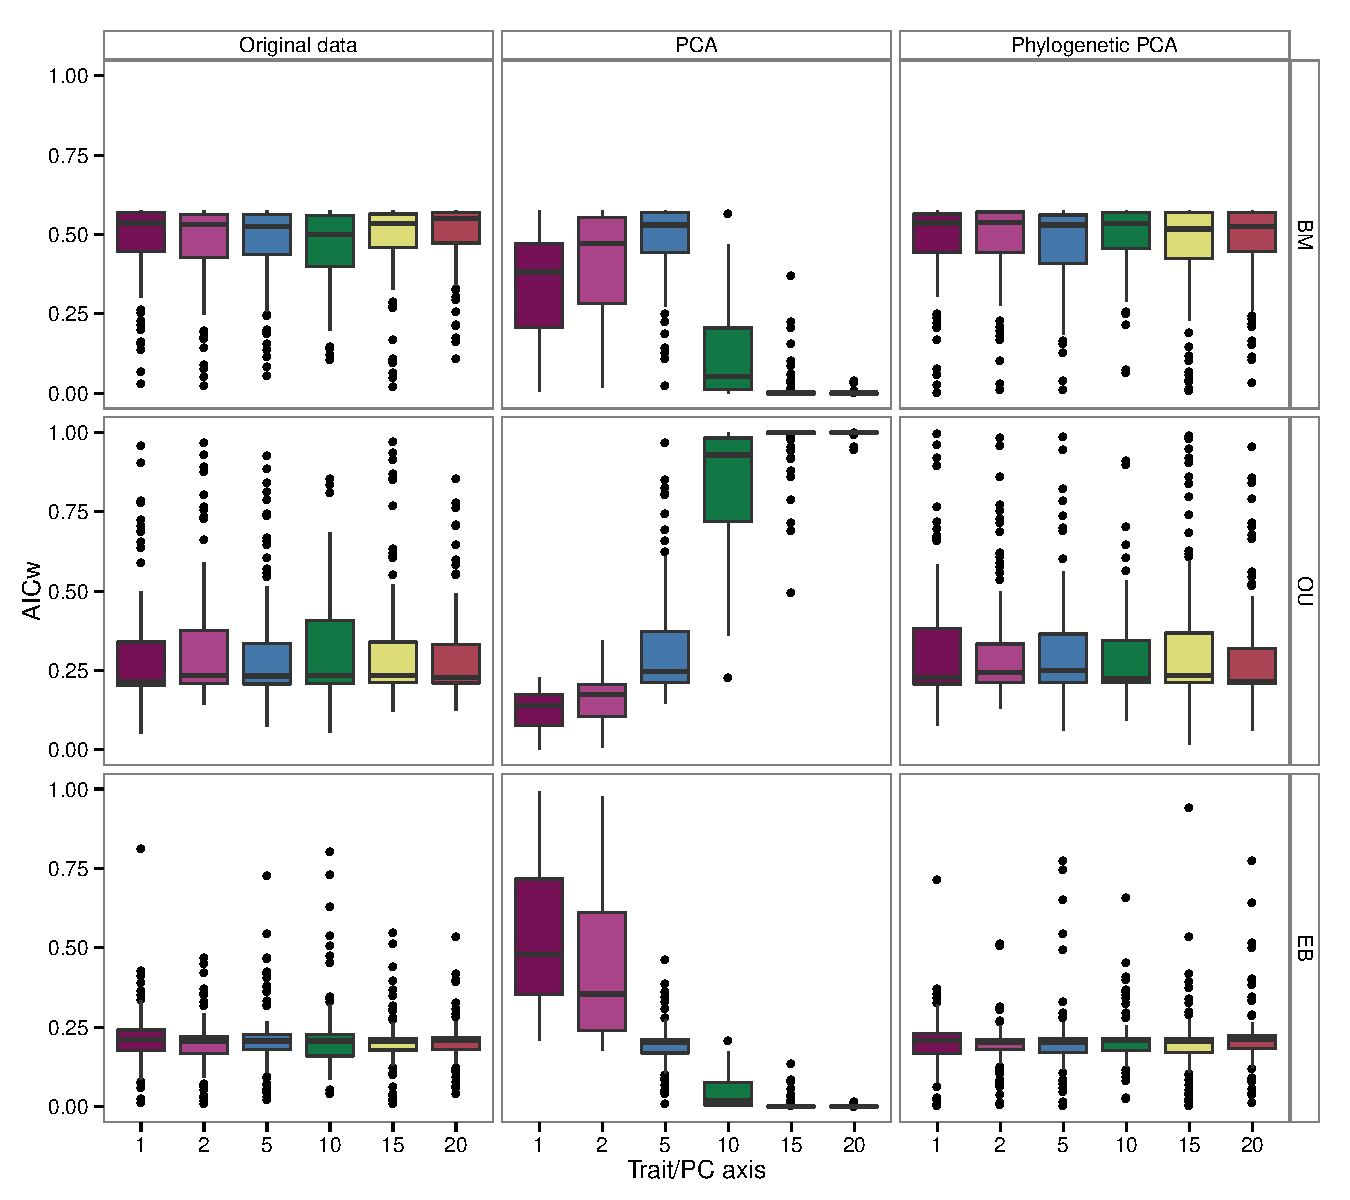
\includegraphics[scale=0.65]{./fig/box-aicw-corbm.pdf}
\caption{Distribution of Akaike weights for the Brownian motion (top row), Ornstein--Uhlenbeck (middle row) or Early--Burst model (bottom row). Models were fit to each replicated dataset for each of 6 different traits which were taken either from the original data (left column), PC scores (middle column) or phylogenetic PC scores (right column). Boxplots indicate the distribution of Akaike weights across each of 100 replicated datasets. Note that EB models have higher Akaike weights for the first few PCs of standard PCA, and that later PCs subsequently favor BM and finally, OU models. No such bias is found across traits for either the original data or pPCA.}
\label{corbm}
\end{figure}

\begin{figure}[p]
\centering
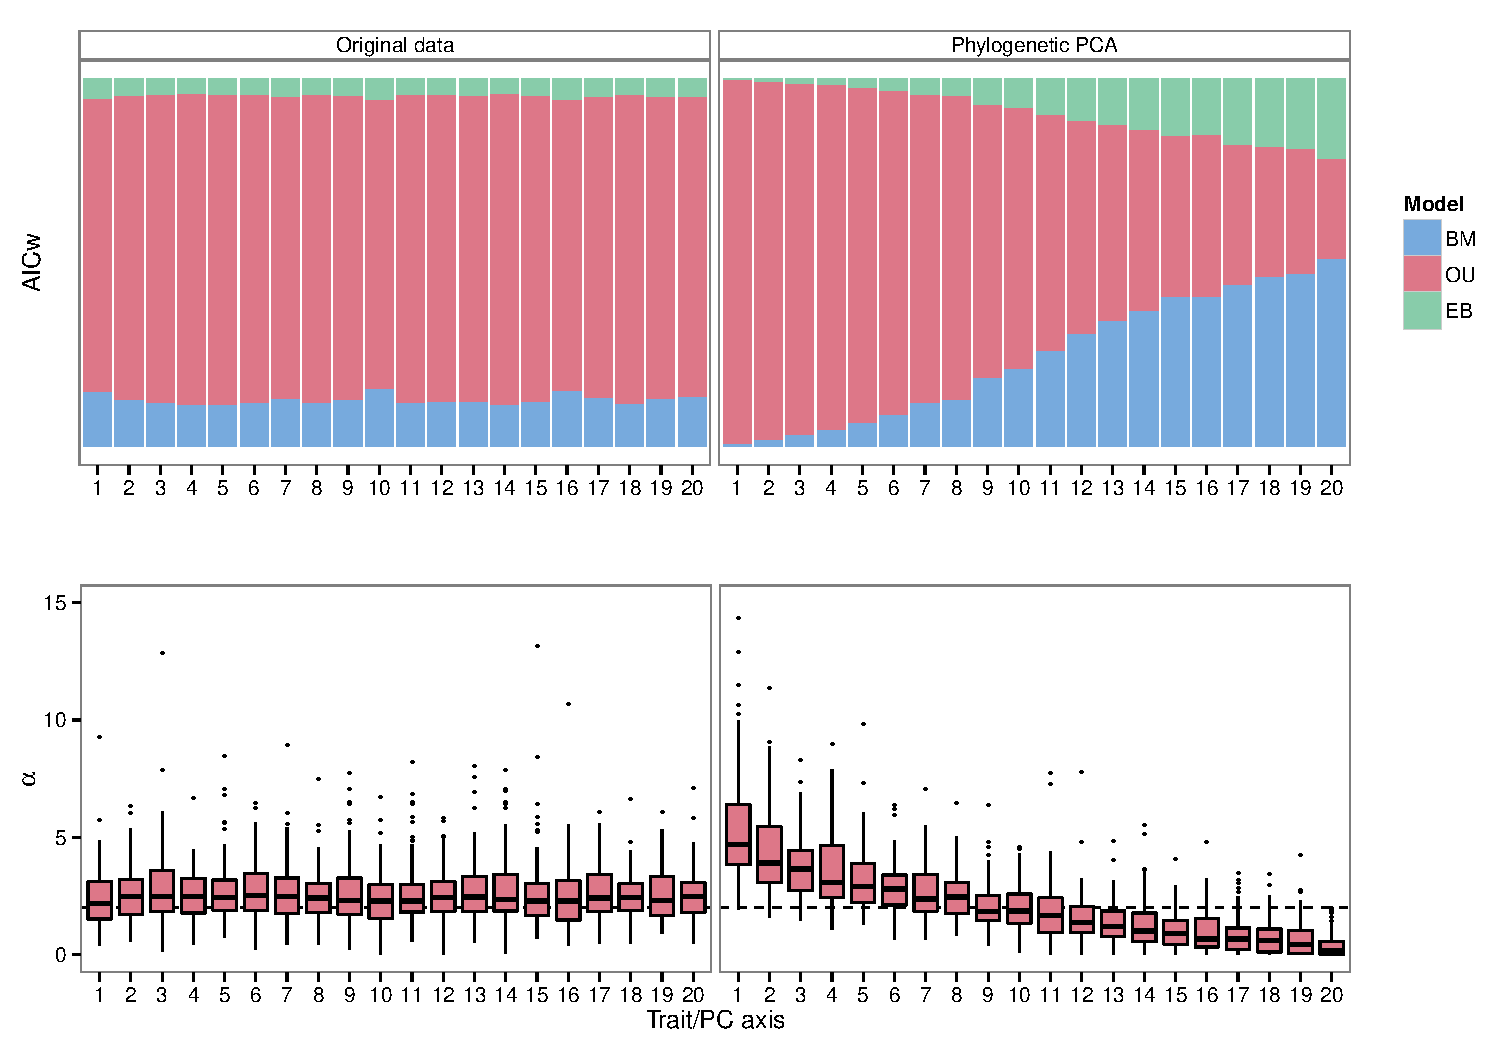
\includegraphics[scale=0.6]{./fig/model-support-alpha.pdf}
\caption{Akaike weights and parameter estimates for data simulated under an OU model, but subsequently fit to pPCA scores assuming multivariate BM. Akaike weights across traits (either original data, or pPCs) show a regular pattern of increasing support for BM and EB  moving down pPCA axes (top panel). Furthermore, while $\alpha$ and other parameters are well--estimated for the original traits, pPCA produces a regular pattern of decreasing $\alpha$ values across pPC scores (bottom panel). Note that the first few pPC axes have strong support for an OU model, and substantially higher estimates of $\alpha$ relative to the value used to generate the data (solid blue line, $\alpha = 2$).}
\label{oufit}
\end{figure}

\begin{figure}[p]
\centering
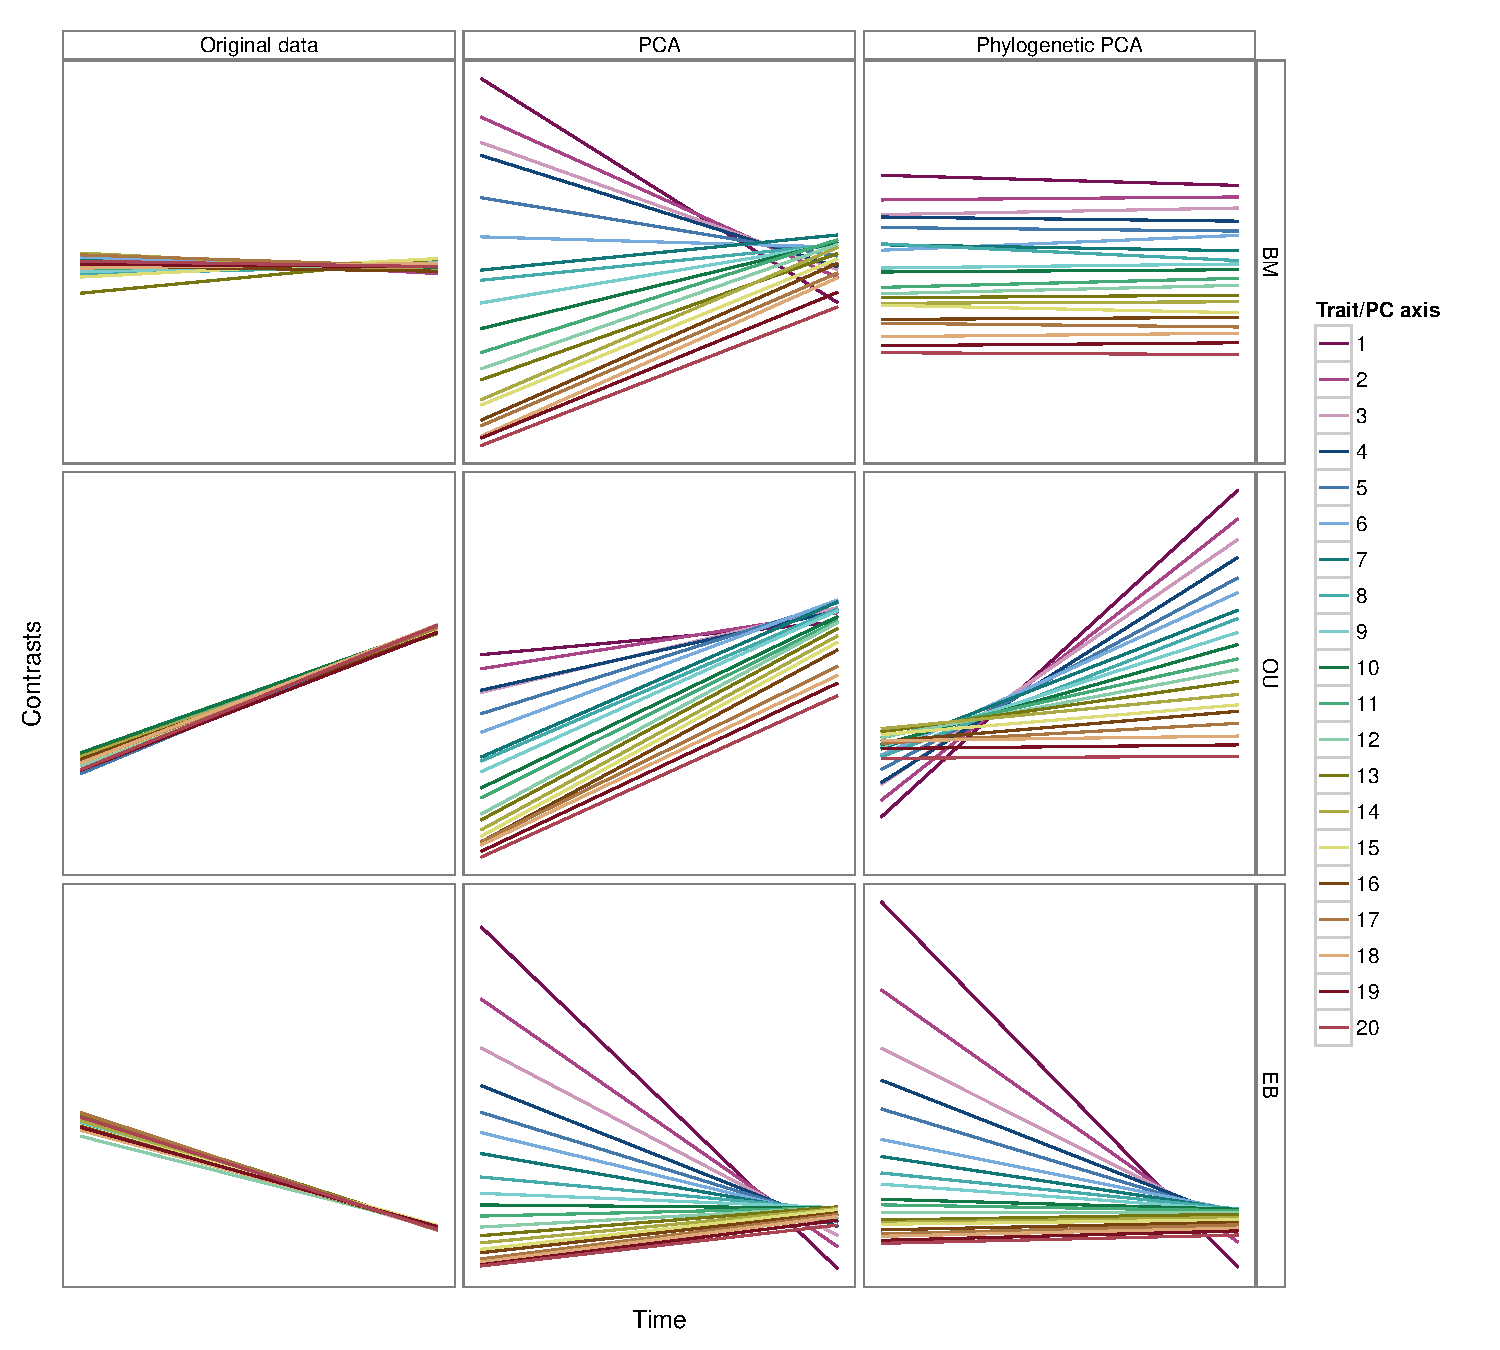
\includegraphics[scale=0.65]{./fig/nh-3models.pdf}
\caption{Relationship between the average phylogenetic independent contrasts and the height of the node across 100 datasets simulated under either a BM (top row), OU (middle row) or EB (bottom row) model of evolution. Contrasts were calculated for each of the 20 traits corresponding to either the original data (left column), PC scores (middle column) or pPPC scores (right column). Each line represents a best--fit linear model to the aggregated data across all 100 replicate simulations. The plots are oriented so that the left side of each panel corresponds to the root of the phylogeny, with time increasing tipward to the right. PCA results in a predictable pattern of increasing slope in the contrasts across PCs. By contrast, pPCA only has systematic distortions across pPC axes when the underlying model is not multivariate BM. When this occurs, the first few pPC axes tend to have more extreme slopes than the original data (but in the correct direction).}
\label{nhplot}
\end{figure}

\begin{figure}[p]
\centering
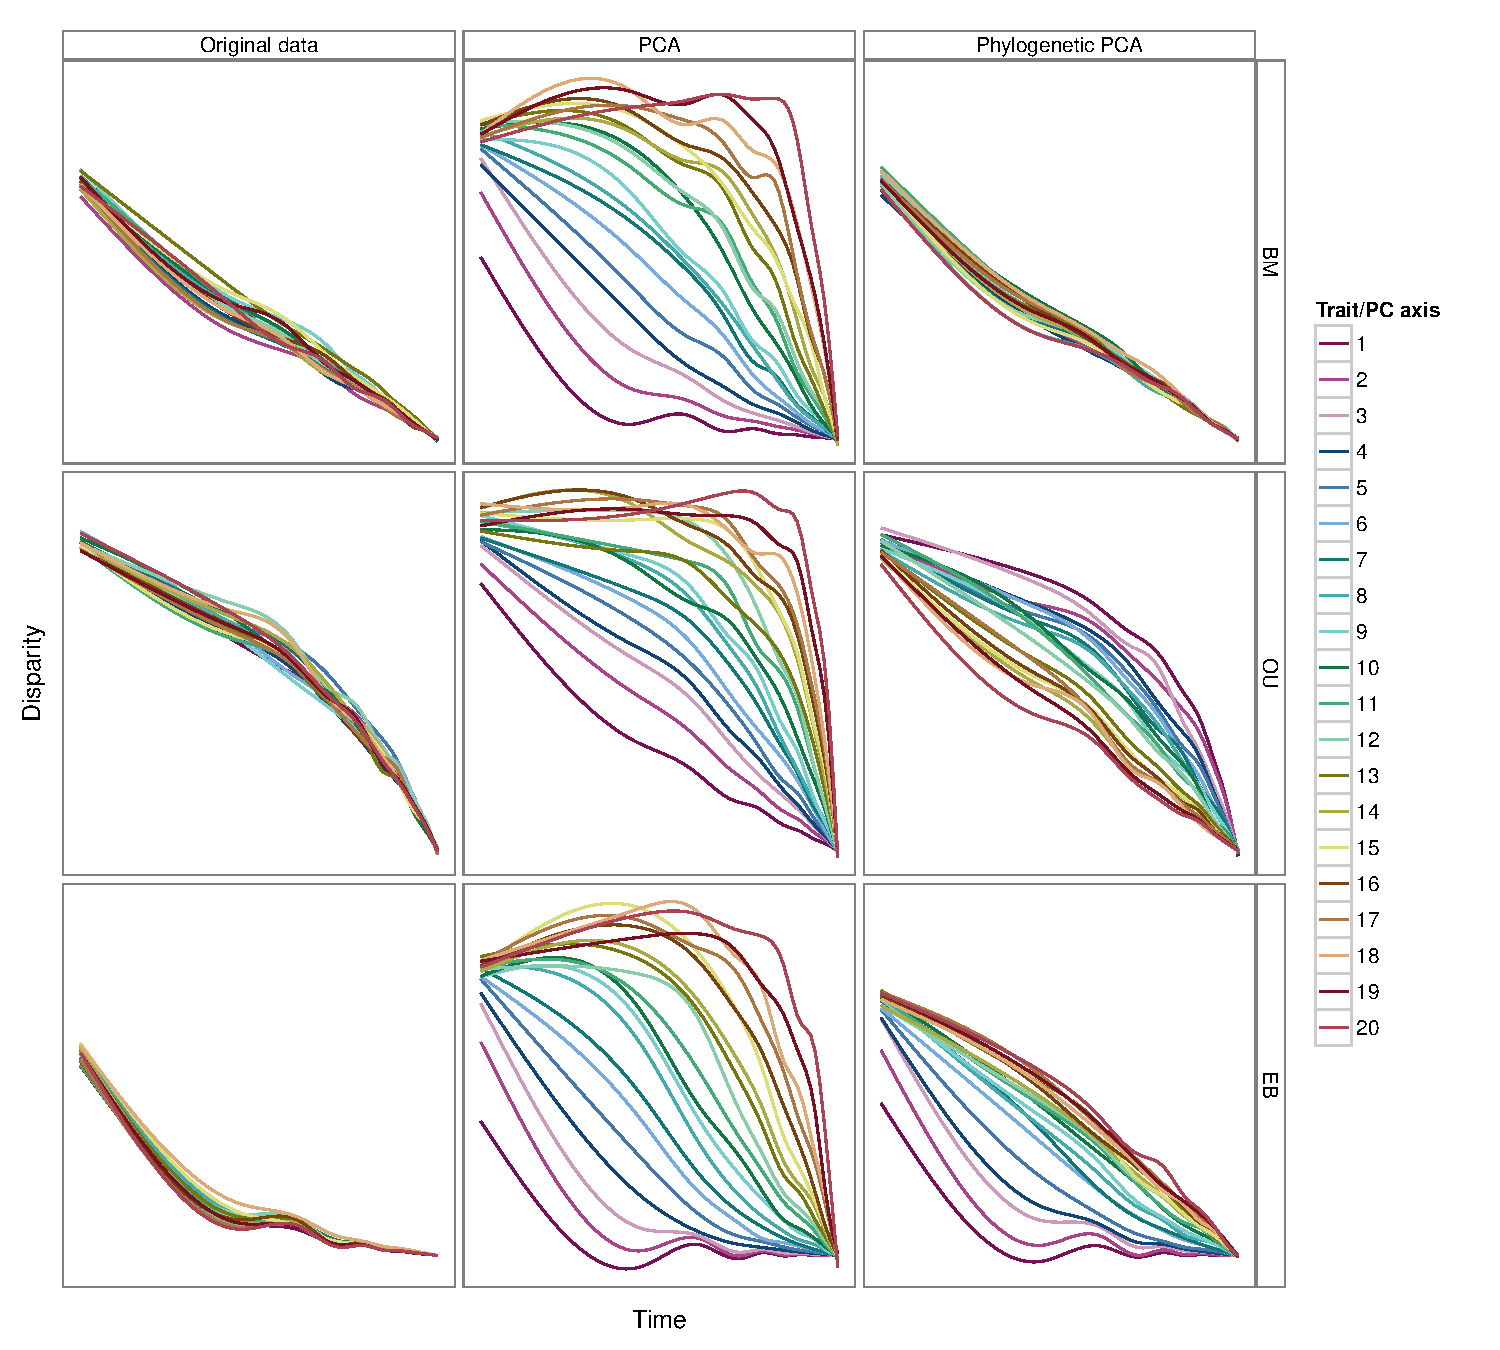
\includegraphics[scale=0.65]{./fig/dtt-3models.pdf}
\caption{Relative disparity through time for the same simulated datasets as in Figure \ref{nhplot}.}
\label{dttplot}
\end{figure}

\renewcommand\thefigure{S\arabic{figure}}
\renewcommand\thetable{S \arabic{table}}
\setcounter{figure}{0}    
\setcounter{table}{0}

\begin{figure}[p]
\centering
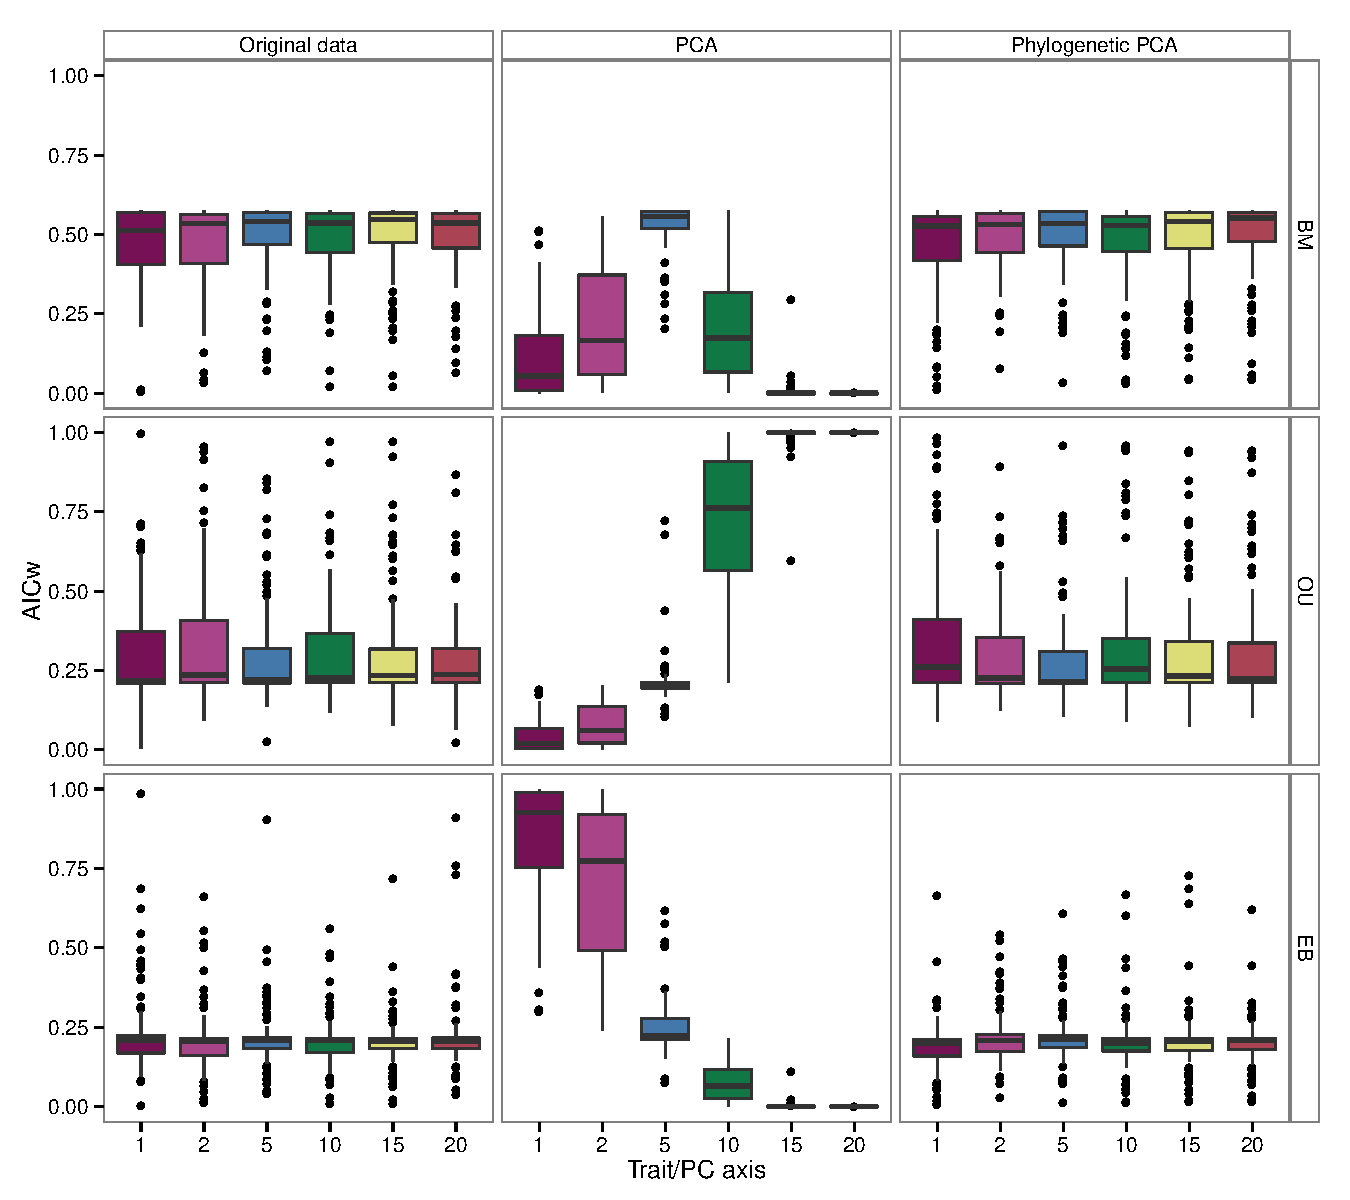
\includegraphics[scale=0.65]{./fig/box-aicw-mvbm.pdf}
\caption{Model support from uncorrelated BM}
\label{aicwbm}
\end{figure}

\begin{figure}[p]
\centering
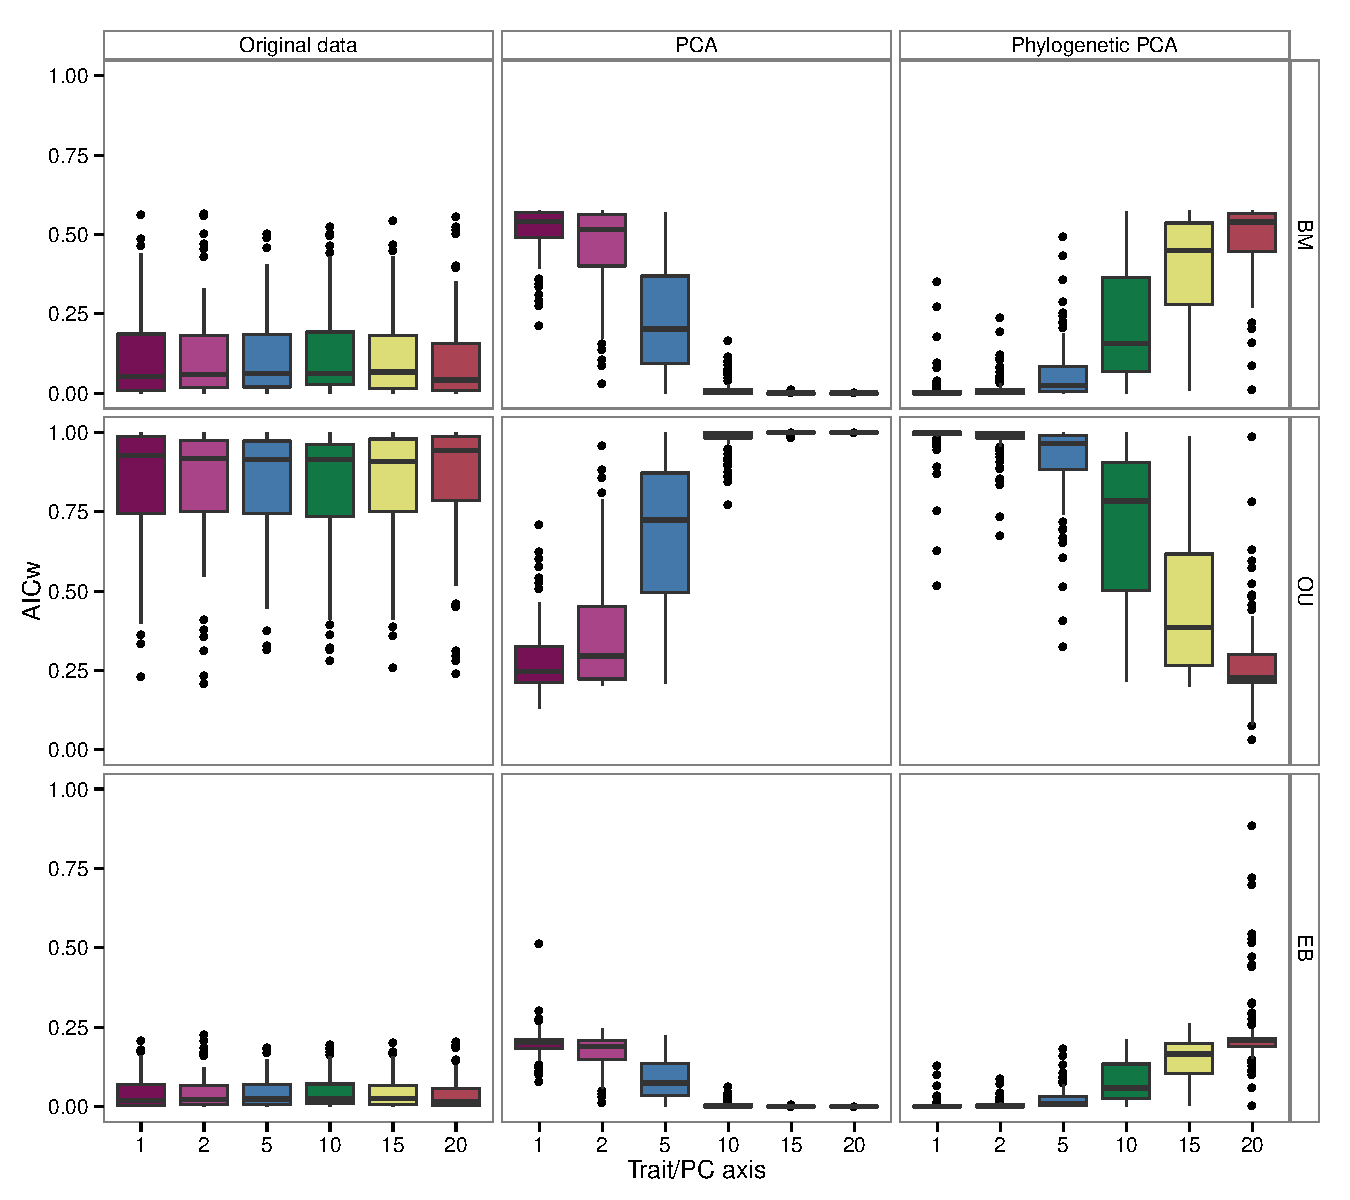
\includegraphics[scale=0.65]{./fig/box-aicw-mvou.pdf}
\caption{Model support from uncorrelated OU}
\label{aicwou}
\end{figure}

\begin{figure}[p]
\centering
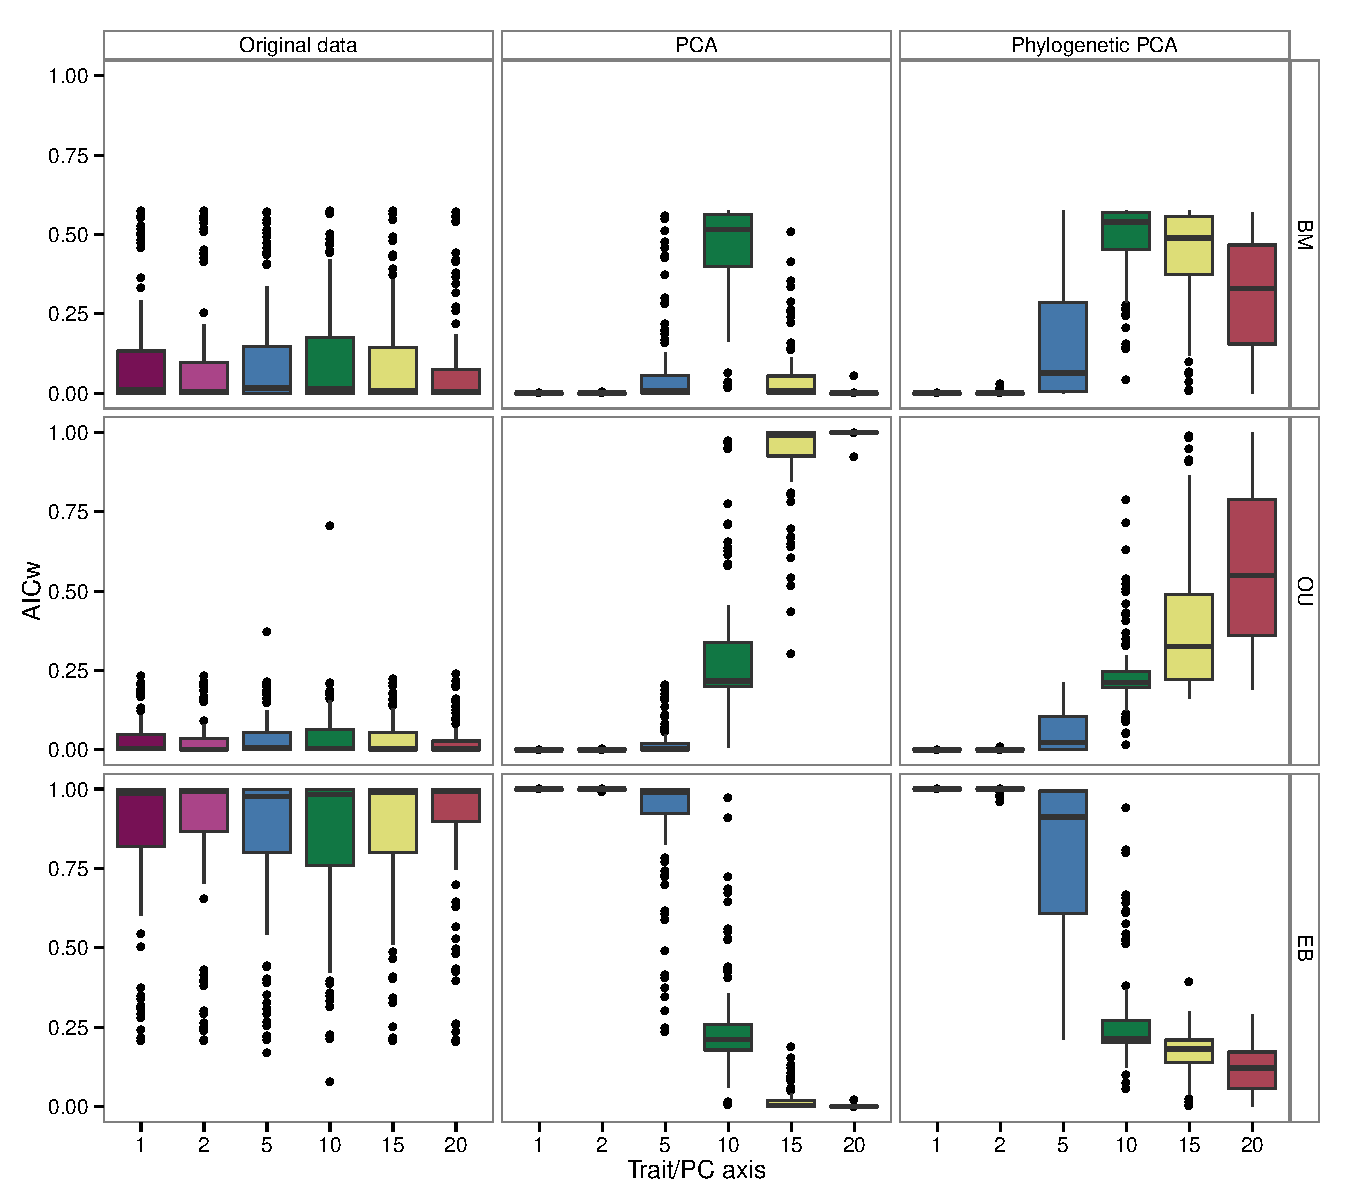
\includegraphics[scale=0.65]{./fig/box-aicw-mveb.pdf}
\caption{Model support from uncorrelated EB}
\label{aicweb}
\end{figure}




\end{document}
